% If enabled, this produces a notes-free version for handing out
%\def\HANDOUT{}
% If enabled in tandem with \HANDOUT, doesn't reformat the slides to fit on a
% single page
%\def\EMAILEDCOPY{}

% The paper: https://arxiv.org/pdf/2508.07177
% Using pympress to present, I think

\documentclass[
    aspectratio=169,
    \ifdefined\HANDOUT
    handout
    \else
    \fi
]{beamer}
\usetheme{AnnArbor}
\usecolortheme{illini}
\setbeamertemplate{note page}[]
\ifdefined\HANDOUT
\ifdefined\EMAILEDCOPY
\else
\usepackage{pgfpages}
\pgfpagesuselayout{resize to}[letterpaper,border shrink=2mm, landscape]
\fi
\else
\setbeameroption{show notes}
\setbeameroption{show notes on second screen=bottom}
\fi
\setbeamertemplate{caption}[numbered]

% Automatically add Section Title Slids
\AtBeginSection[]{
  \begin{frame}
  \vfill
  \centering
  \begin{beamercolorbox}[sep=8pt,center,shadow=true,rounded=true]{title}
    \usebeamerfont{title}\insertsectionhead\par%
  \end{beamercolorbox}
  \vfill
  \end{frame}
}

%TODO Font should be adjusted (bigger)
\usepackage[]{amsfonts}
\newcommand{\overbar}[1]{\mkern 1.5mu\overline{\mkern-1.5mu#1\mkern-1.5mu}\mkern 1.5mu}
\usepackage{amsmath}
\usepackage{amssymb}
\usepackage{mathtools}
\usepackage{listings}
\usepackage{algorithm}
\usepackage{algpseudocode}
\usepackage{ulem}
\usepackage{censor}

%\usepackage{biblatex}
%\renewcommand*{\bibfont}{\small}

\DeclareMathOperator*{\argmax}{arg\,max}
\DeclareMathOperator*{\argmin}{arg\,min}

\graphicspath{img}

\title[PHYS 595]{``An Analogy of Frequency Droop Control for Grid-forming Sources'' Lu, '25, arXiv}
\subtitle{A PHYS 595 Journal Club Presentation}
\author[ES]{Eric Silk}
\institute[ECE@UIUC]{Electrical and Computer Engineering\linebreak University of Illinois at Urbana-Champaign}
\date{April 24th, 2026}
\logo{
\includegraphics[height=1cm]{img/small_logo.png}}
\begin{document}
\definecolor{UIUCOrange}{RGB}{255,95,5}
\definecolor{UIUCBlue}{RGB}{19,41,75}
\definecolor{UIUCBlueSubhead}{RGB}{5,86,165}
\definecolor{UIUCBlueKnockoutheader}{RGB}{32,64,151}
\definecolor{UIUCGray1}{RGB}{232,233,234}
\definecolor{UIUCGray2}{RGB}{166,168,171}
\definecolor{UIUCGray3}{RGB}{94,102,105}

\begin{frame}
    \titlepage
    \tiny
    Compiled: \today
    \note[item]{Mention I use to work with the second author}
\end{frame}


\section{Background}
\begin{frame}
    \frametitle{Paper Motivation}
    \begin{itemize}
        \item Principally pedagogical
        \item Mechanical analogy for electrical system
        \item Useful for education and intuition when designing power systems
        \item Not research, \textit{per se}
    \end{itemize}
    \note[item]{These papers aren't uncommon in engineering as "support" for new research areas}
    \note[item]{Given the emphasis on broad interest/Accessibility in this class, this seemed appropriate}
\end{frame}

\begin{frame}
    \frametitle{Power Generation: Historical Perspective}
    \begin{columns}
        \begin{column}{0.5\textwidth}
            \begin{itemize}
                \item Power is alternating current (AC)
                \item Historically highly centralized
                \item Uses \textit{synchronous machines}
                \item System frequency is proportional to power balance
                \item Strong coupling between grid dynamics and generator behavior
            \end{itemize}
        \end{column}
        \begin{column}{0.5\textwidth}
            \begin{figure}[h]
                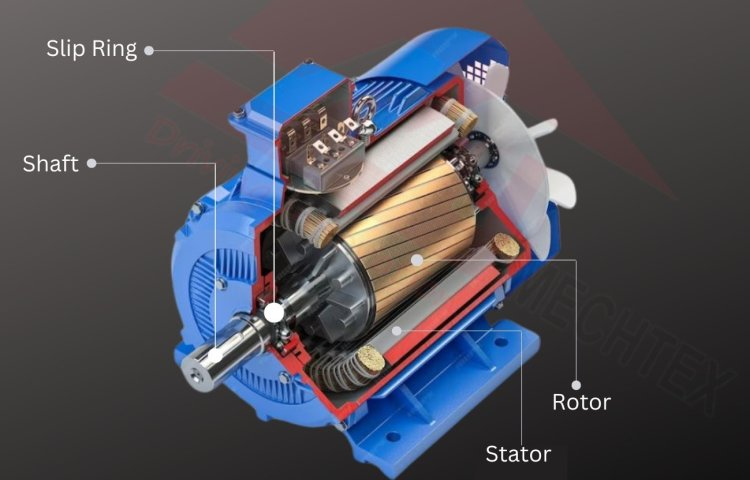
\includegraphics[width=0.9\textwidth]{img/synch_machine.jpg}
                \caption{A cutaway render of a synchronous machine\cite{synch_machine}}
            \end{figure}
        \end{column}
    \end{columns}

    \note[item]{Centralized due to economies of scale}
    \note[item]{The strong coupling is bidirectional}
\end{frame}

\begin{frame}
    \frametitle{Primary Control of Synchronous Machines}
    \begin{columns}
        \begin{column}{0.5\textwidth}
            \begin{itemize}
                \item Inverse relationship between frequency and speed
                \item Droop control
                \item Prevents frequency collapse (or the opposite)
                \item Enables power sharing between generators
                \item ``Grid forming'' (GFM) resources
            \end{itemize}
            \vspace{10pt}
            \begin{equation}
                f = f_{nom}-m_p\left(P-P_{ref}\right),\ 
                m_p\coloneqq \frac{\Delta f}{S_{rated}}
            \end{equation}
            where $f$ is frequency, $P$ is active power, $(\cdot)_{nom}$ is a nominal quantity,
            $S_rated$ is the rated apparent power.
        \end{column}
        \begin{column}{0.5\textwidth}
            \begin{figure}[h]
                \vspace{-10pt}
                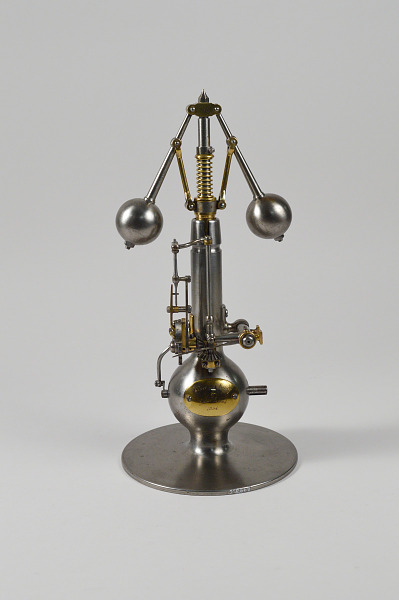
\includegraphics[height=0.6\textheight]{img/guvnah.jpg}
                \caption{An early form of primary control: a steam engine governor\cite{guvnah}}
            \end{figure}
        \end{column}
    \end{columns}

    \note[item]{We need controls to keep system frequency at nominal}
    \note[item]{Primary control is a form of proportional control}
    \note[item]{Prevents runaway, but doesn't remove frequency error entirely}

\end{frame}

\begin{frame}
    \frametitle{Inverter Based Resources: The Future of Generation}
    \begin{columns}
        \begin{column}{0.5\textwidth}
            \begin{itemize}
                \item Some resources produce \textit{direct} current (DC)
                \item This must be converted to AC via \textit{inverters}
                      \begin{itemize}
                          \item Known as "Inverter-based resources" (IBR)
                      \end{itemize}
                \item Historically ``grid following'' (GFL), converting to GFM
                \item Weakly coupled to grid dynamics
            \end{itemize}
        \end{column}
        \begin{column}{0.5\textwidth}
            \begin{figure}[h]
                \vspace{-10pt}
                \includegraphics[height=0.6\textheight]{img/solar_panels.png}
                \caption{An example of an IBR}
            \end{figure}
        \end{column}
    \end{columns}
    \note[item]{Think of inverters like digital to analog converters}
    \
    \note[item]{GFL's just do whatever the grid is doing using PLL's}
    \note[item]{GFM's try to act more like synchronous generators}
    \note[item]{Weakly coupled $\implies$ inverters can sort of do whatever they want}
    \note[item]{This freedom makes control development harder}
    \note[item]{But this freedom also creates opportunities}
\end{frame}


\section{Key Results}
\subsection{The Analogy}
\begin{frame}
    \begin{block}{Question}
        \begin{center}
            How can we reframe these abstract/hard to visualize electrical quantities?
        \end{center}
    \end{block}
    \begin{block}{Answer}\pause
        \begin{center}
            Convert them by mathematical analogy to some \textit{physical} system
        \end{center}
    \end{block}
\end{frame}
\begin{frame}
    \frametitle{Basic Visual}
    \begin{figure}[h]
        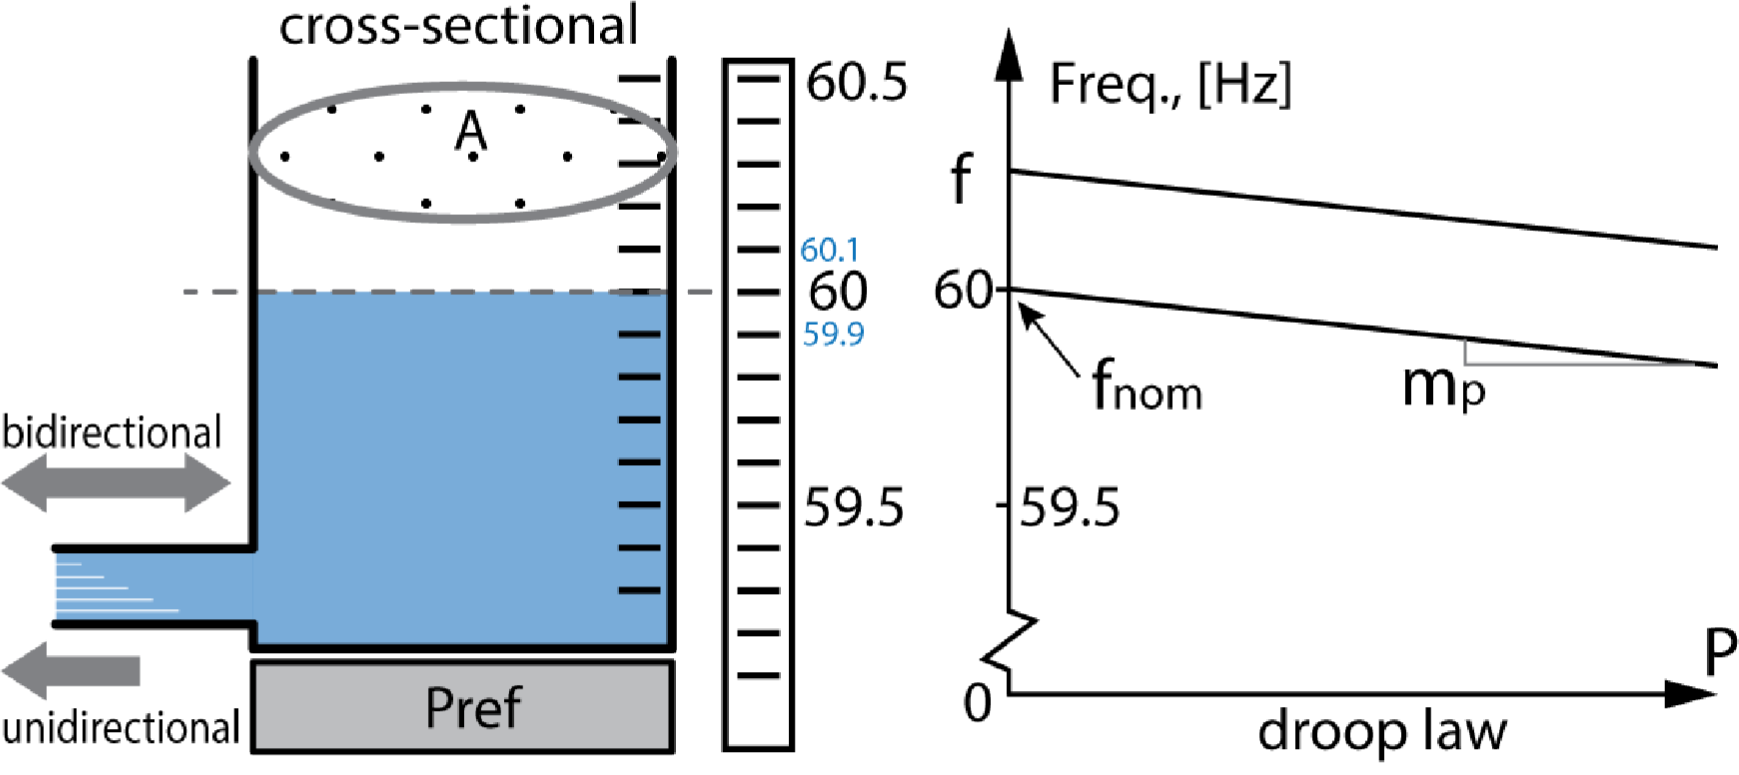
\includegraphics[width=0.85\textwidth]{img/physical_analogy.png}
        \caption{The basic analogy, with the associated droop curve\cite{main_paper}}
    \end{figure}
    \note[item]{Visualize droop as a water tank}
    \note[item]{Water level is frequency}
    \note[item]{The area is the reciprocal of the droop coefficient/slope (and vice-versa)}
    \note[item]{An adjustable block is the setpoint}
    \note[item]{Pipes $\iff$ cables}
\end{frame}

\begin{frame}
    \frametitle{Comparable Values}
    \begin{table}[]
        \begin{tabular}{l|ll}
            Symbol    & Communicating Vessels                     & GFM sources        \\ \hline
            $f$       & \multicolumn{1}{l|}{Water Level}          & Actual Frequency   \\
            $f_{nom}$ & \multicolumn{1}{l|}{Base Reference Level} & Nominal Frequency  \\
            $A$       & \multicolumn{1}{l|}{Cross-sectional Area} & Reciprocal of m\_p \\
            $m_p$     & \multicolumn{1}{l|}{Reciprocal of A}      & Droop slope        \\
            $P$       & \multicolumn{1}{l|}{Outflow Water Amount} & Real Power         \\
            $P_{ref}$ & \multicolumn{1}{l|}{Block Elevation}      & Power Setpoint     \\
            $L$       & \multicolumn{1}{l|}{Pipes}                & Electrical Cables
        \end{tabular}
    \end{table}
\end{frame}

\begin{frame}
    \frametitle{Nonlinear Controls}
    \begin{figure}[h]
        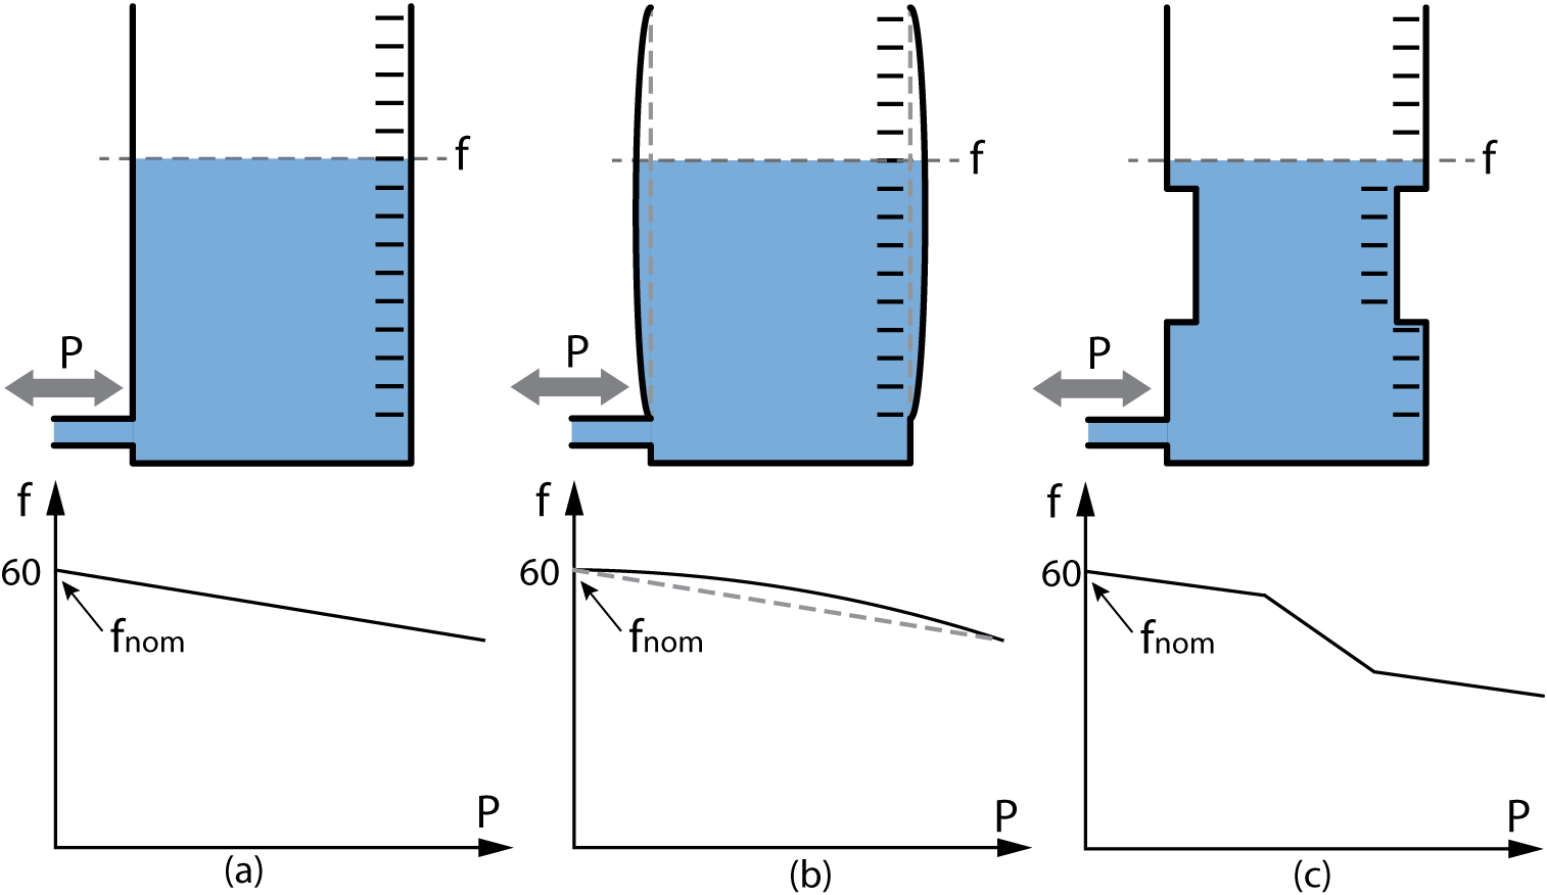
\includegraphics[height=0.7\textheight]{img/nonlinear.png}
        \caption{Various droop shapes: Linear (a), convex curved (b), and piecewise linear (c)\cite{main_paper}}
    \end{figure}
    \note[item]{We can extend the basic analogy (leftmost) to include nonlinear
        (center) and piecewise linear (right) droop controls}
    \note[item]{The shape of the droop curve closely relates to the shape of the tank}
\end{frame}

\subsection{Applications/Demonstration}
\begin{frame}
    \frametitle{Power Setpoints and Grid Connection}
    \begin{figure}[h]
        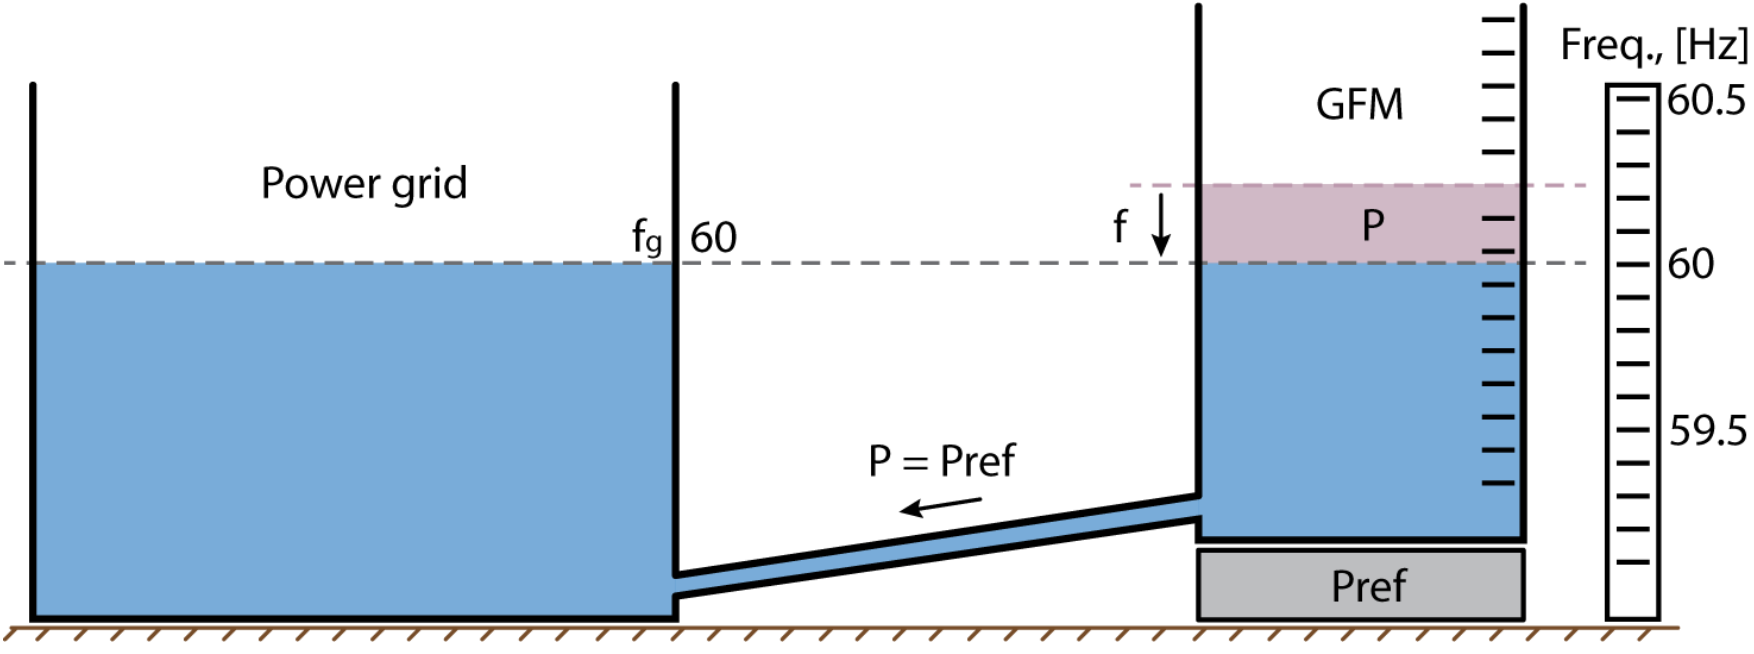
\includegraphics[height=0.65\textheight]{img/grid_connected.png}
        \caption{A local GFM tied to the bulk grid\cite{main_paper}}
    \end{figure}
    \note[item]{The bulk grid can generally be seen as an exceedingly large tank}
    \note[item]{To some degree, the GFM can do whatever it wants and $f$ will stay at $f_{nom}$}
\end{frame}
\begin{frame}
    \frametitle{Interconnected GFM Resources}
    \begin{figure}[h]
        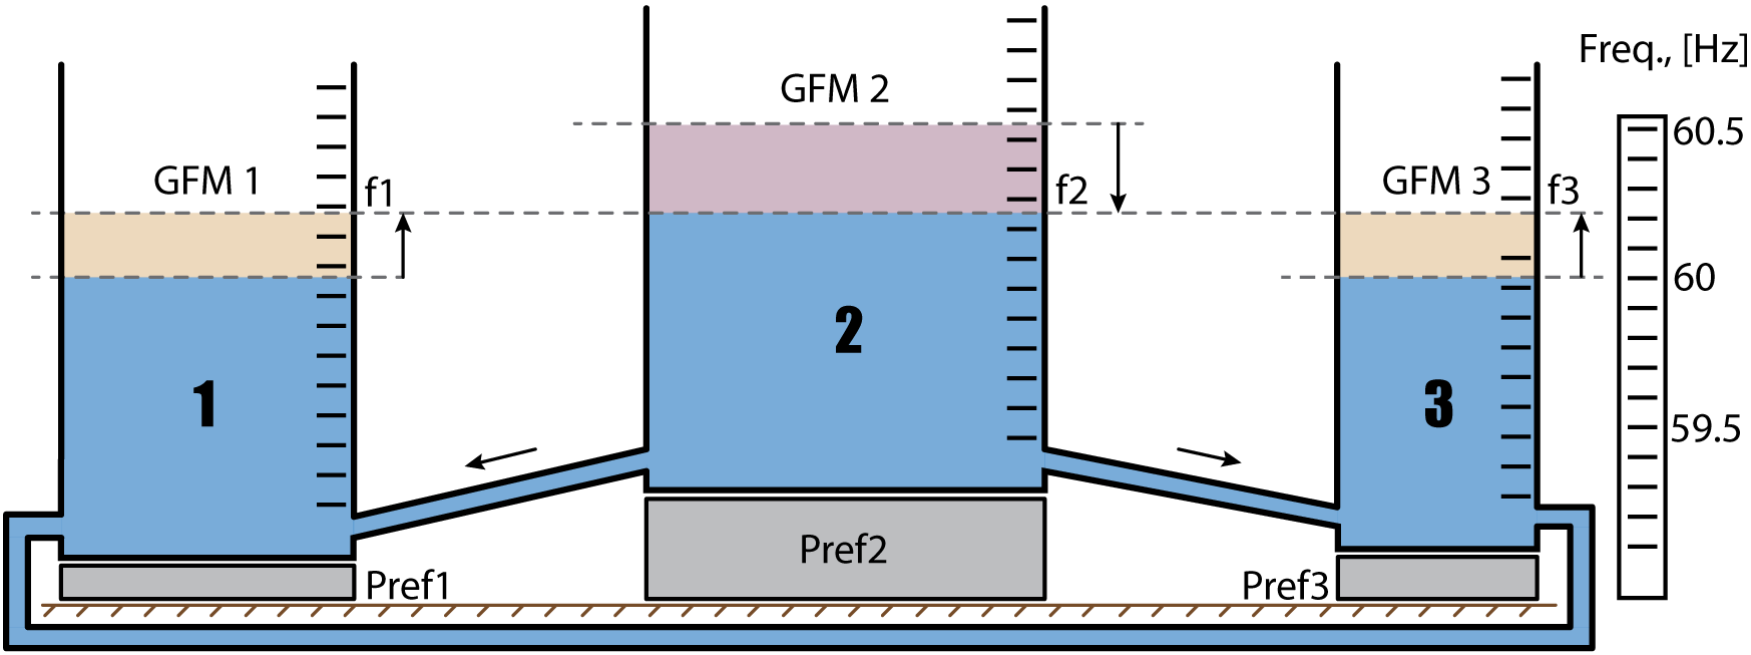
\includegraphics[height=0.65\textheight]{img/interconnected.png}
        \caption{Frequency regulation/power sharing among interconnected resources\cite{main_paper}}
    \end{figure}
    \note[item]{An example of how multiple GFM's can be connectd in this analogy}
    \note[item]{Note that different tank areas and references change how they share the load}
    \note[item]{Also note that the cross-sectional area is not typically configurable}
\end{frame}
\begin{frame}
    \frametitle{Microgrid}
    \begin{figure}[h]
        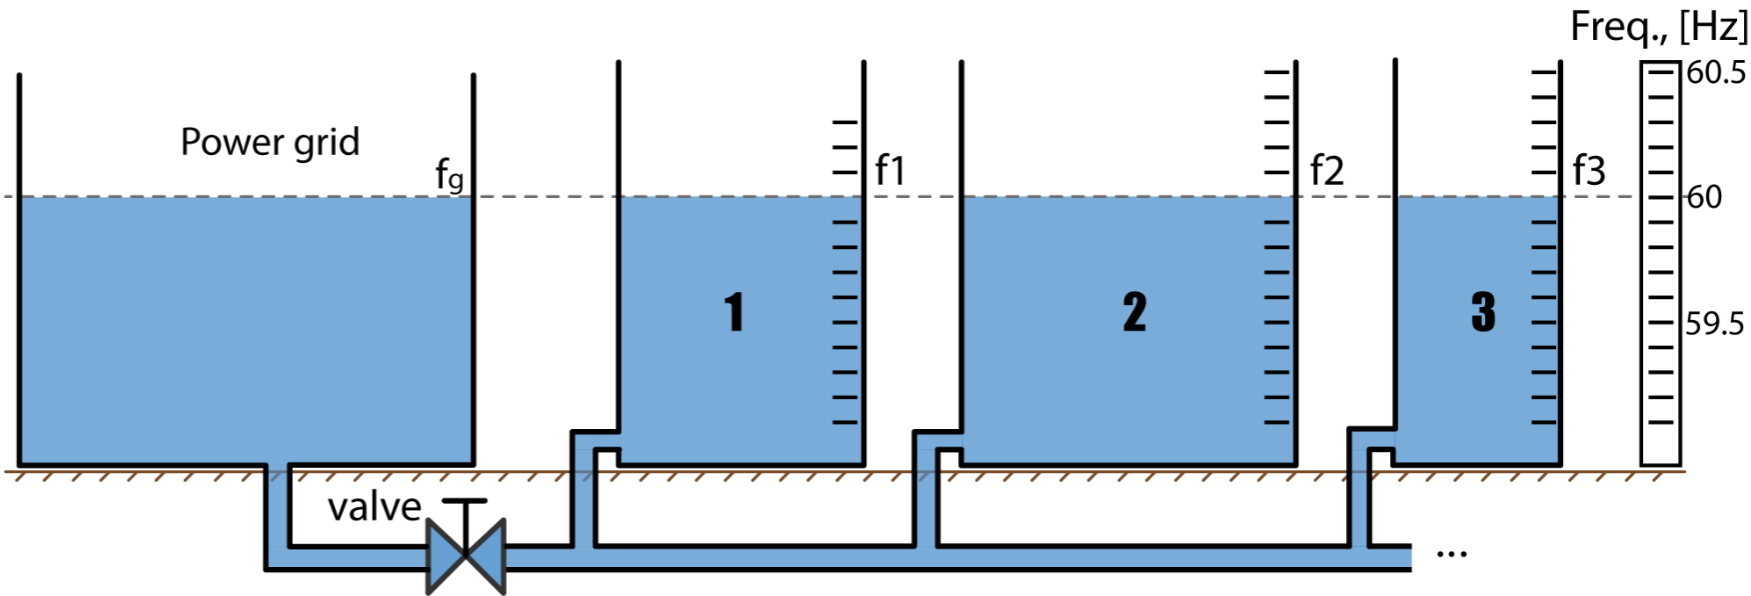
\includegraphics[height=0.65\textheight]{img/microgrid.png}
        \caption{An example microgrid, showing the ability to island via a valve\cite{main_paper}}
    \end{figure}
    \note[item]{This example extends the prior one by introducing a valve -- a way to island}
\end{frame}

\begin{frame}
    \frametitle{Numerical Results Presented in the Paper}
    \begin{columns}
        \begin{column}{0.5\textwidth}
            \begin{itemize}
                \item Several numerical simulations included
                \item Ultimately, nothing surprising here
            \end{itemize}
        \end{column}
        \begin{column}{0.5\textwidth}
            \begin{figure}[h]
                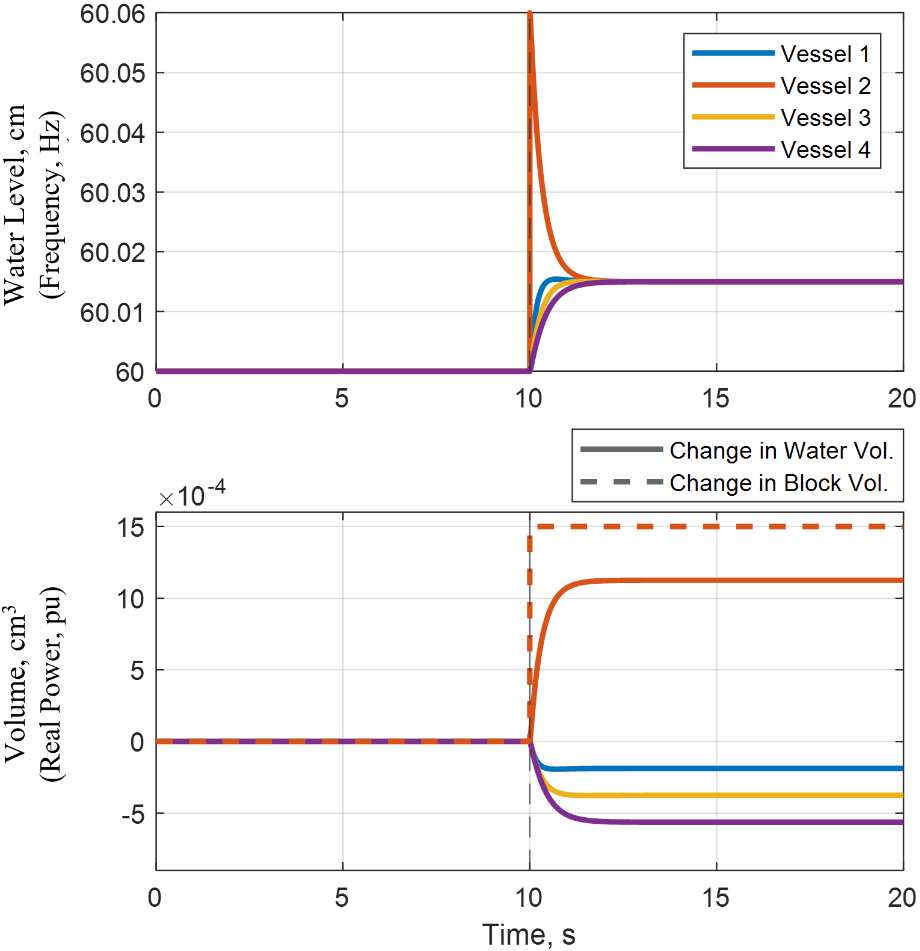
\includegraphics[height=0.5\textheight]{img/numerical.png}
                \caption{Simulation of changing the power/block setpoint\cite{synch_machine}}
            \end{figure}
        \end{column}
    \end{columns}
    \note[item]{The paper also includes several numerical examples, one of which is shown here}
    \note[item]{We're not going to dwell on this because they're all exactly as one might expect}
    \note[item]{Numerical examples rely on the mathematical descriptions, abstracted from physical realities}
    \note[item]{Which leads into my critical feedback...}
\end{frame}

\section{Critical Response}
\begin{frame}
    \frametitle{Importance}
    \begin{columns}
        \begin{column}{0.5\textwidth}
            \begin{block}{Negatives}
                \begin{itemize}
                    \item Water-tank analogy already exists for droop control in synchronous machines
                    \item IBR droop control is designed to be identical
                    \item Analogy for GFM's is thus trivial
                    \item Unclear how this might help understand other controls (dVOC, etc.)
                \end{itemize}
            \end{block}
        \end{column}
        \begin{column}{0.5\textwidth}
            \begin{block}{Positives}
                \begin{itemize}
                    \item The nonlinear/piecewise linear examples are perhaps not obvious
                    \item Could be a useful for new researchers in this space
                    \item Old results, but with new language and examples
                \end{itemize}
            \end{block}
        \end{column}
    \end{columns}
    \note[item]{Obviously, one would expect an analogy for device A to work for
        device B if device B is designed to behave exactly like A}
    \note[item]{The extension to include nonlinear/piecewise linear is perhaps non-obvious}
    \note[item]{Its important to sometimes re-embed concepts into popular
        conciousness, even if they're well-established}
    \note[item]{Using new language/examples for old knowledge is useful}
    \note[item]{Imagine if all our amplifier design textbooks still used vacuum tubes!}
\end{frame}

\begin{frame}
    \frametitle{Broad Interest and Accessibility}
    \begin{columns}
        \begin{column}{0.5\textwidth}
            \begin{block}{Positives}
                \begin{itemize}
                    \item Extremely approachable analogy
                    \item Good visuals and examples
                    \item Modifications to base example laid out logically
                \end{itemize}
            \end{block}
        \end{column}
        \begin{column}{0.5\textwidth}
            \begin{block}{Negatives}
                \begin{itemize}
                    \item Insufficent background for non-power audience
                    \item Insufficient motivation for alternative controls
                \end{itemize}
            \end{block}
        \end{column}
    \end{columns}
    \note[item]{ODE's are often introduced using waterflow analogy -- it's super intuitive!}
    \note[item]{Almost all the visuals are well created and presented}
    \note[item]{Paper proceeds in an orderly fashion, gradually adding complexity}
    \note[item]{But...not enough background for non-power engineers (and definitely not non-EE)}
    \note[item]{Insufficient motivation for why we would use droop in GFM's}
\end{frame}

\section{Conclusion}
\begin{frame}
    \frametitle{Concluding Remarks}
    \begin{columns}
        \begin{column}{0.5\textwidth}
            \begin{itemize}
                \item Power generation is switching to IBRs
                \item IBRs are switching to GFMs
                \item GFMs may use linear, piecewise linear, nonlinear droop, and others
                \item Water tank analogy
            \end{itemize}
        \end{column}
        \begin{column}{0.5\textwidth}
            \begin{itemize}
                \item Trivial extension of existing pedagogy
                \item Insufficent background
                \item Approachable analogy
                \item Exising analogy in new language
            \end{itemize}
        \end{column}
    \end{columns}
\end{frame}
\begin{frame}
    \frametitle{Bibliography}
    \bibliographystyle{amsalpha}
    {
        \bibliography{qual_presentation.bib}
    }
\end{frame}
\begin{frame}
    \begin{center}
        \vspace{20pt}
        {
            \Huge
            Q\&A
        }
    \end{center}
\end{frame}

\end{document}